\documentclass[a4paper]{article}

%% Language and font encodings
\usepackage{appendix}
\usepackage[english]{babel}
\usepackage[utf8x]{inputenc}
\usepackage{natbib}
  \setcitestyle{open={(},close={)}}
\usepackage{indentfirst}
\usepackage[T1]{fontenc}
\usepackage{enumitem}


%\usepackage{datetime}
\usepackage[nodayofweek,level]{datetime}

\usepackage{amsmath}
\usepackage{amsfonts}
\usepackage{amssymb}
\usepackage{graphicx}
\usepackage{booktabs}
\usepackage{float}
\usepackage{multirow}
\usepackage{subcaption}
\usepackage{threeparttable}
\usepackage{pdflscape}
\usepackage{lscape}
\usepackage{array} % for defining a new column type
\usepackage{tabulary}
\newcolumntype{K}[1]{>{\centering\arraybackslash}p{#1}}
\usepackage{animate}
\DeclareMathOperator*{\argmax}{arg\,max}
\DeclareMathOperator*{\argmin}{arg\,min}
\usepackage{siunitx}
\usepackage{gensymb} % degree symbol \degree

\makeatletter
\newcommand{\leqnos}{\tagsleft@true\let\veqno\@@leqno}
\newcommand{\reqnos}{\tagsleft@false\let\veqno\@@eqno}
\reqnos
\makeatother


\newdate{date}{30}{07}{2022}
\date{\displaydate{date} }

%% Sets page size and margins
\usepackage[a4paper,top=3cm,bottom=2cm,left=3cm,right=3cm,marginparwidth=1.75cm]{geometry}

%% Useful packages
\usepackage{amsmath}
\usepackage{amssymb}
\usepackage{graphicx}
\usepackage[colorinlistoftodos]{todonotes}
\usepackage[colorlinks=true, allcolors=blue, backref=page]{hyperref}
\usepackage{setspace}
\setlength{\parindent}{0pt}
\setlength{\parskip}{1em}
\setstretch{1.5}
\usepackage{comment} % package to selectively include/exclude portions of text
\usepackage{setspace} % The \addlinespace command is part of the "setspace" package in LaTeX.


\title{\LARGE JOB LOSS}

\begin{document}

\maketitle

\section{Descriptive analysis}\label{sec:desc_pam}

\begin{tabular}{lc}
\multicolumn{2}{c}{} \\ \hline
 & (1) \\
VARIABLES & job\_loss \\ \hline
 &  \\
position & -0.001*** \\
 & (0.000) \\
signed\_work\_card & 0.001 \\
 & (0.002) \\
hours\_worked & -0.001*** \\
 & (0.000) \\
temporary\_worker = 2 & -0.003*** \\
 & (0.001) \\
educ = 2 & 0.001 \\
 & (0.001) \\
educ = 3 & 0.004*** \\
 & (0.001) \\
educ = 4 & -0.001 \\
 & (0.002) \\
work\_category = 2 & 0.003 \\
 & (0.002) \\
work\_category = 5, omitted & - \\
 &  \\
work\_category = 6, omitted & - \\
 &  \\
monthly\_work\_income & -0.000* \\
 & (0.000) \\
urbana & 0.002 \\
 & (0.041) \\
job\_start & 0.019*** \\
 & (0.000) \\
year\_quarter = 20122 & 0.039*** \\
 & (0.001) \\
year\_quarter = 20123 & 0.060*** \\
 & (0.002) \\
year\_quarter = 20124 & 0.091*** \\
 & (0.002) \\
year\_quarter = 20131 & 0.111*** \\
 & (0.002) \\
year\_quarter = 20132 & 0.125*** \\
 & (0.002) \\
year\_quarter = 20133 & 0.141*** \\
 & (0.002) \\
year\_quarter = 20134 & 0.170*** \\
 & (0.002) \\
year\_quarter = 20141 & 0.183*** \\
 & (0.002) \\
year\_quarter = 20142 & 0.194*** \\
 & (0.003) \\
year\_quarter = 20143 & 0.213*** \\
 & (0.003) \\
year\_quarter = 20144 & 0.243*** \\
 & (0.003) \\
year\_quarter = 20151 & 0.260*** \\
 & (0.003) \\
year\_quarter = 20152 & 0.278*** \\
 & (0.003) \\
year\_quarter = 20153 & 0.311*** \\
 & (0.003) \\
year\_quarter = 20154 & 0.338*** \\
 & (0.003) \\
year\_quarter = 20161 & 0.363*** \\
 & (0.003) \\
year\_quarter = 20162 & 0.383*** \\
 & (0.003) \\
year\_quarter = 20163 & 0.406*** \\
 & (0.004) \\
year\_quarter = 20164 & 0.443*** \\
 & (0.004) \\
year\_quarter = 20171 & 0.454*** \\
 & (0.004) \\
year\_quarter = 20172 & 0.469*** \\
 & (0.004) \\
year\_quarter = 20173 & 0.487*** \\
 & (0.004) \\
year\_quarter = 20174 & 0.517*** \\
 & (0.004) \\
year\_quarter = 20181 & 0.531*** \\
 & (0.004) \\
year\_quarter = 20182 & 0.542*** \\
 & (0.004) \\
year\_quarter = 20183 & 0.563*** \\
 & (0.004) \\
year\_quarter = 20184 & 0.594*** \\
 & (0.004) \\
year\_quarter = 20191 & 0.606*** \\
 & (0.004) \\
year\_quarter = 20192 & 0.619*** \\
 & (0.004) \\
year\_quarter = 20193 & 0.636*** \\
 & (0.005) \\
year\_quarter = 20194 & 0.674*** \\
 & (0.005) \\
year\_quarter = 20201 & 0.731*** \\
 & (0.005) \\
year\_quarter = 20202 & 0.726*** \\
 & (0.005) \\
year\_quarter = 20203 & 0.723*** \\
 & (0.005) \\
year\_quarter = 20204 & 0.751*** \\
 & (0.005) \\
year\_quarter = 20211 & 0.765*** \\
 & (0.005) \\
year\_quarter = 20212 & 0.773*** \\
 & (0.005) \\
year\_quarter = 20213 & 0.788*** \\
 & (0.006) \\
year\_quarter = 20214 & 0.856*** \\
 & (0.006) \\
year\_quarter = 20221 & 0.866*** \\
 & (0.006) \\
year\_quarter = 20222 & 0.873*** \\
 & (0.006) \\
year\_quarter = 20223 & 0.887*** \\
 & (0.006) \\
 &  \\
Observations & 2,496,247 \\
R-squared & 0.455 \\
Ind FE & Yes \\
Ind FE & Yes \\
 Root mean squared error & 0.207 \\ \hline
\multicolumn{2}{c}{ Standard errors in parentheses} \\
\multicolumn{2}{c}{ *** p$<$0.01, ** p$<$0.05, * p$<$0.1} \\
\end{tabular}


\begin{figure}[hb]
  \centering
  \caption{Job loss work category}
  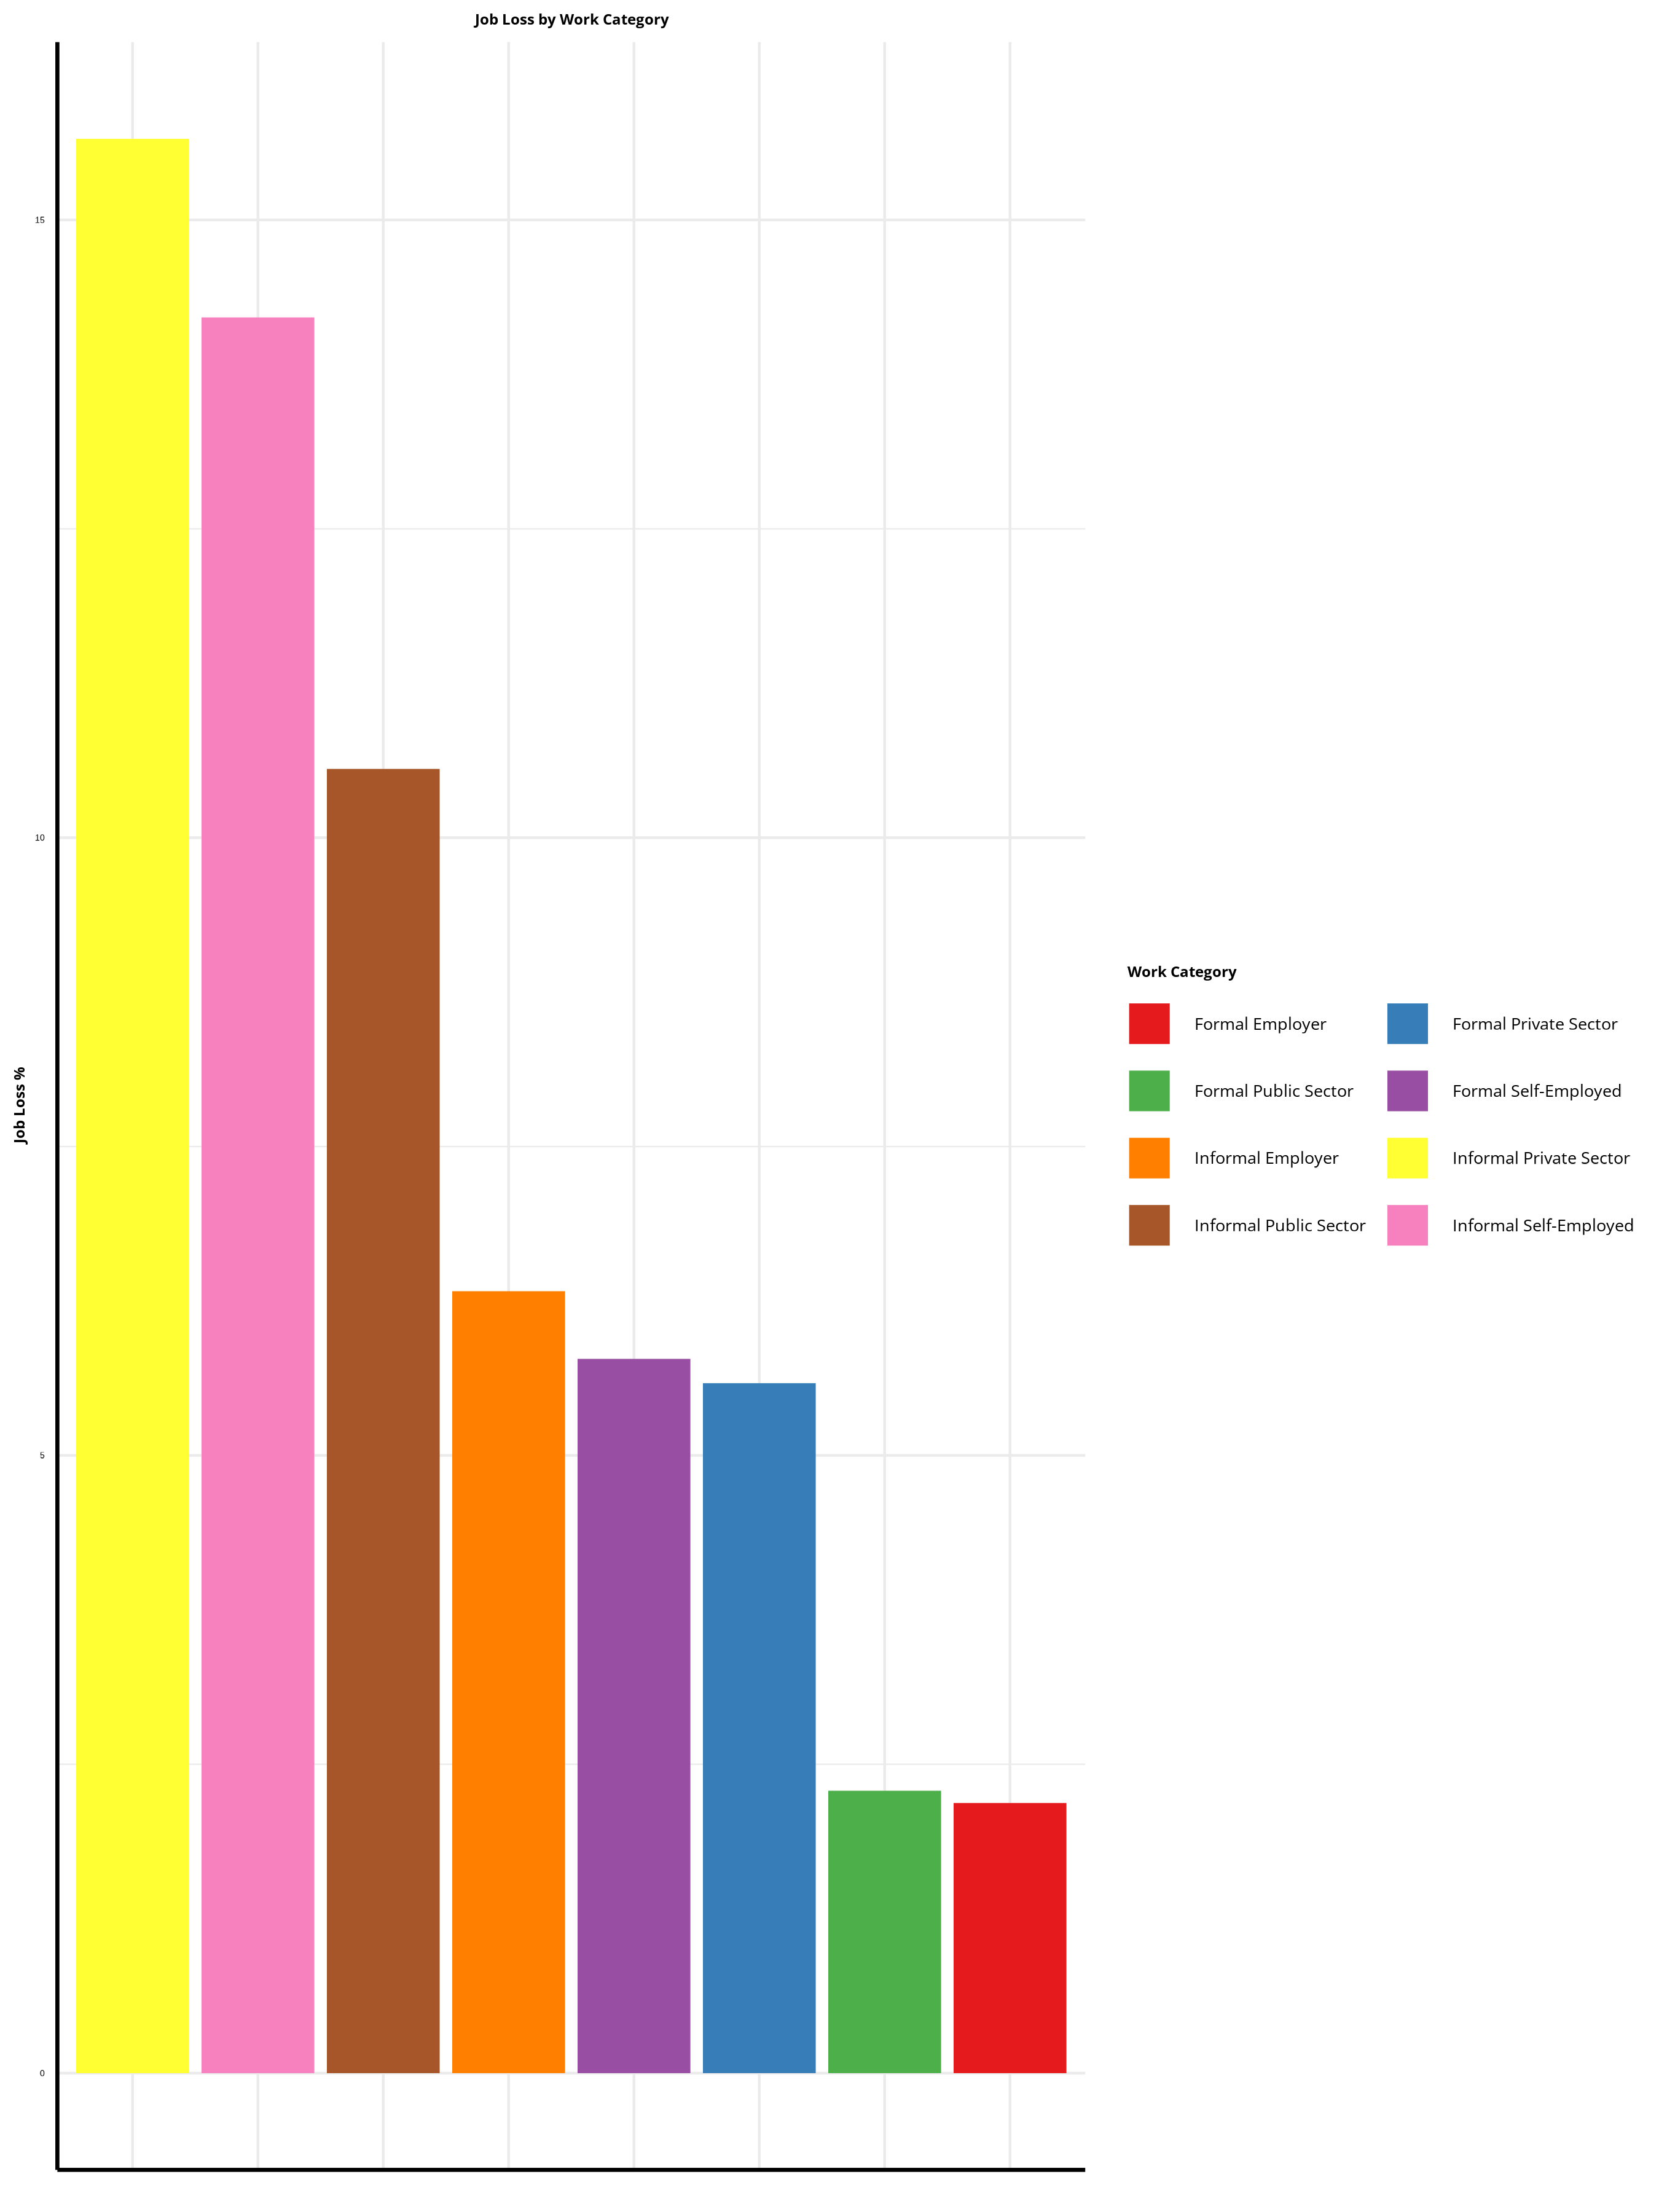
\includegraphics[width=0.85\linewidth]{../analysis/output/graph/_graph_job_loss_work_category.png}
  \label{fig:_graph_job_loss_work_category}
\end{figure}


\begin{figure}[hb]
  \centering
  \caption{Job loss work category}
  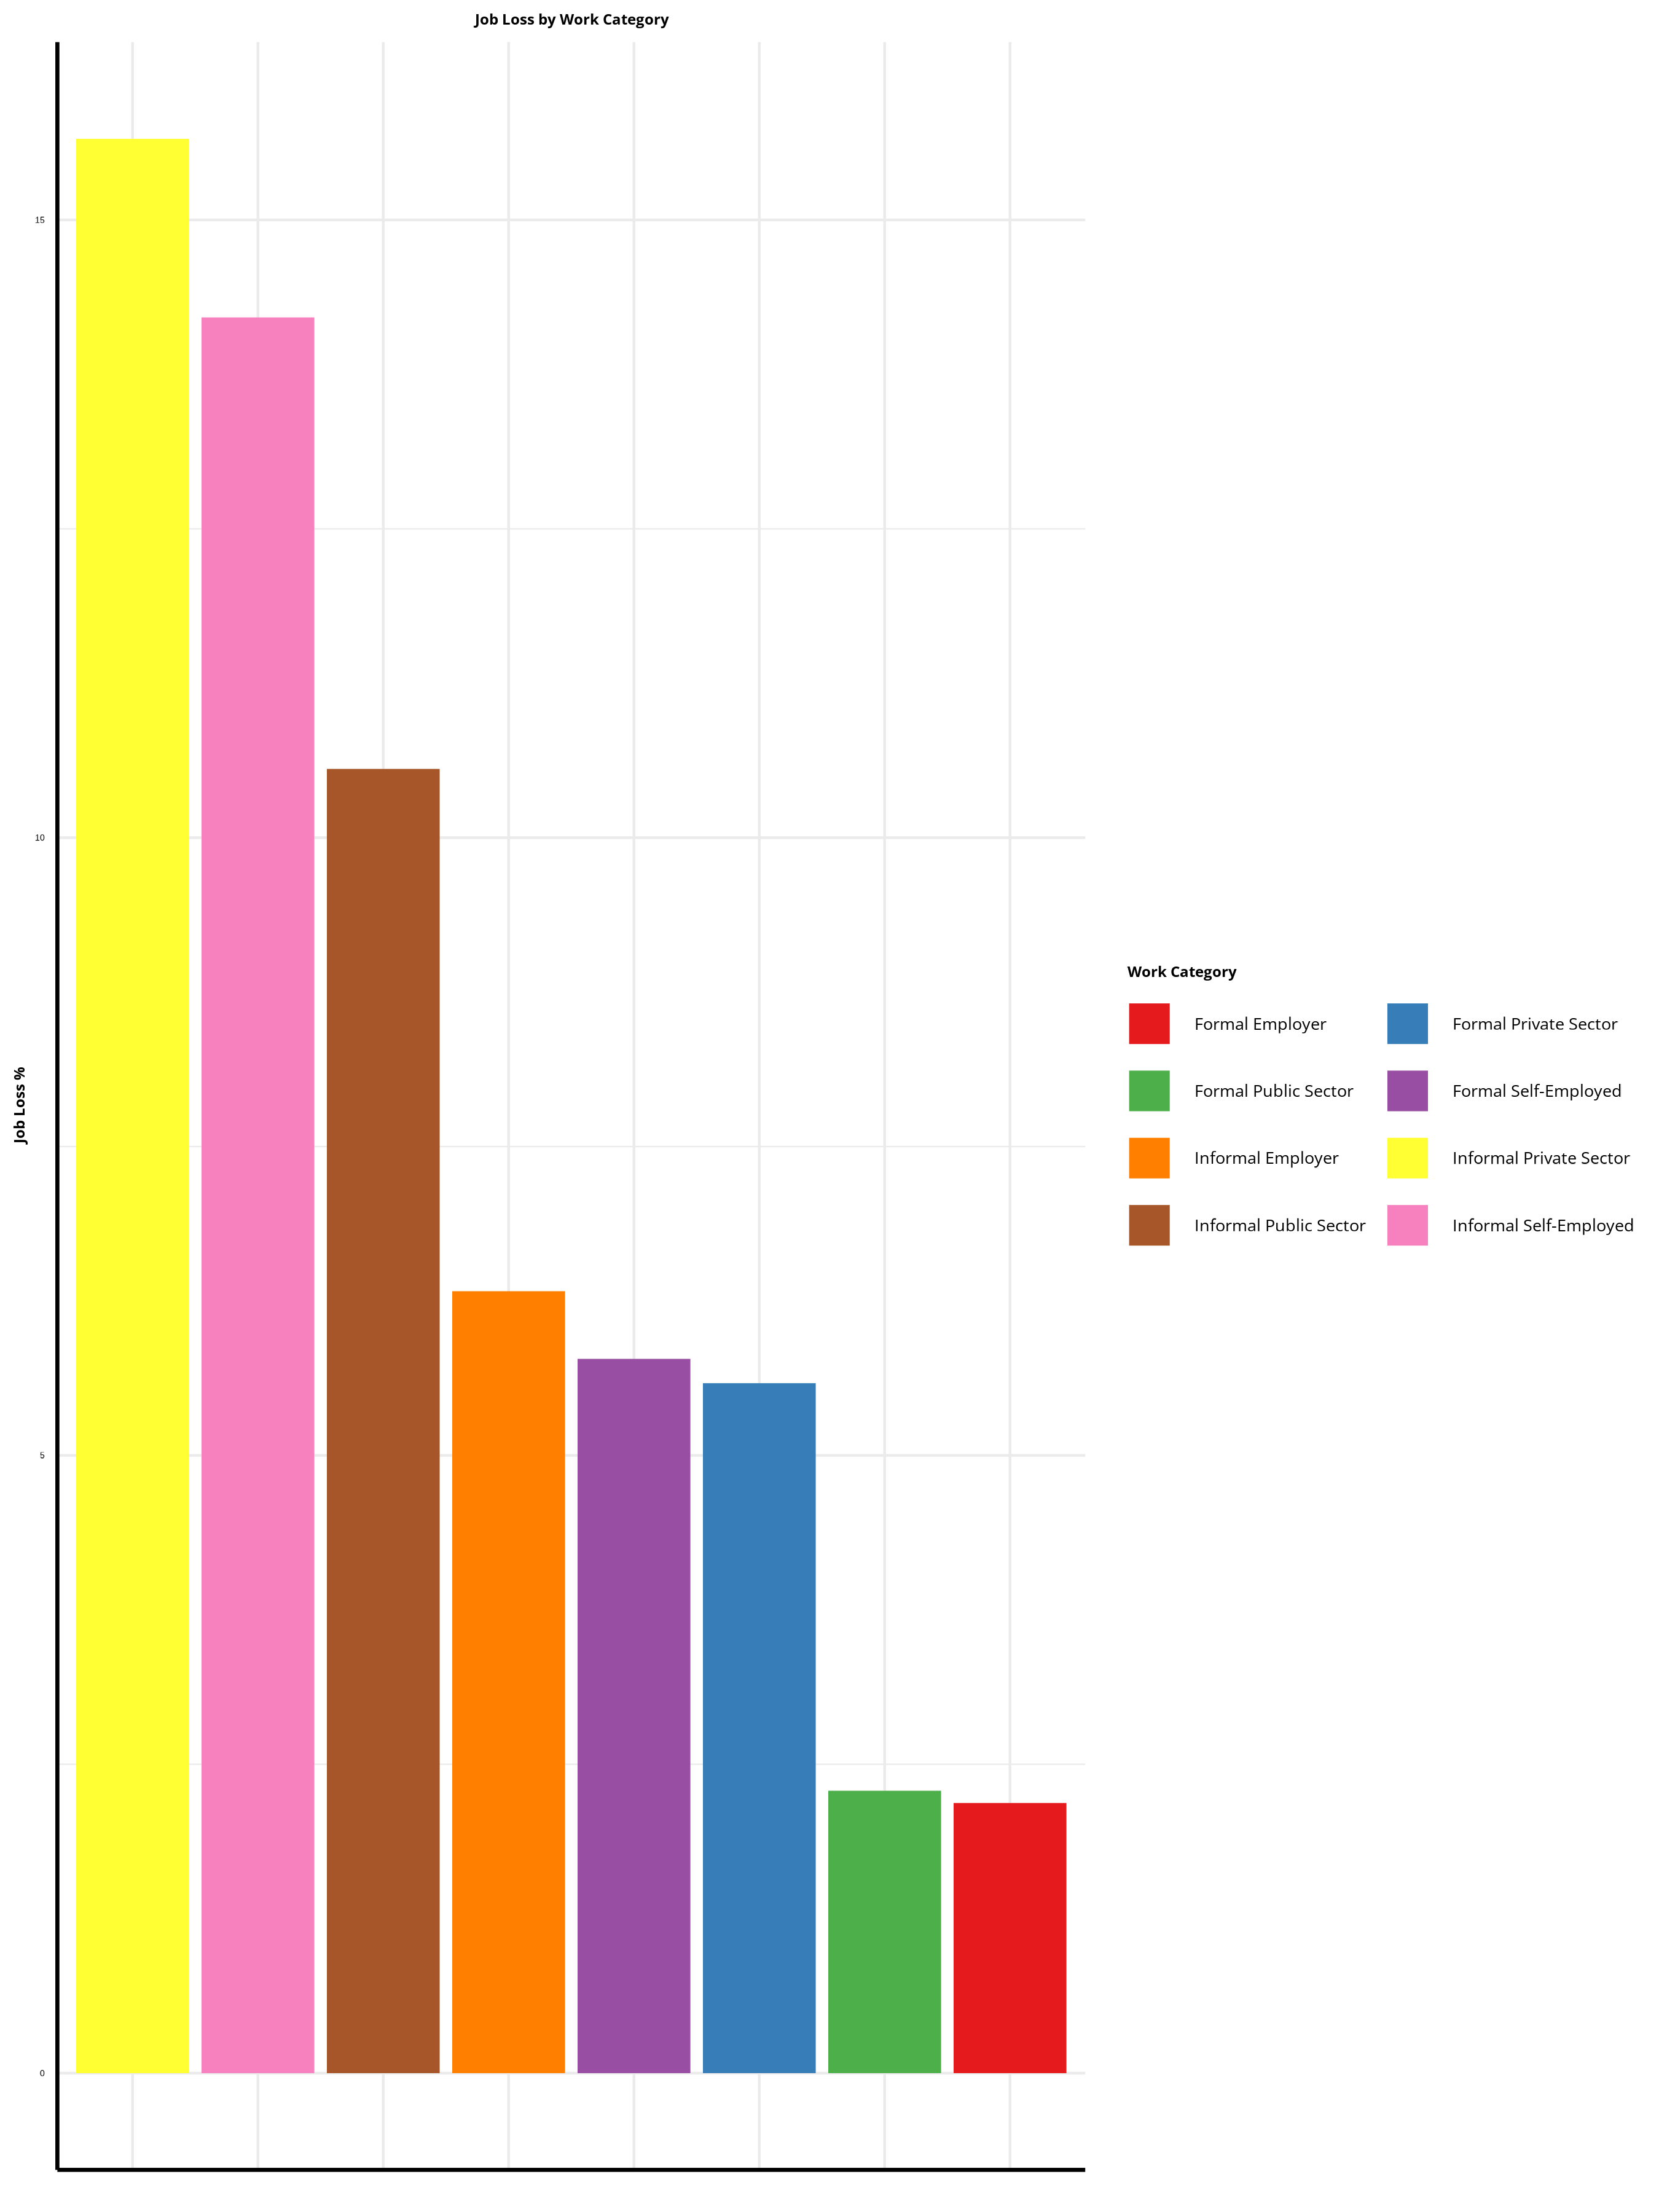
\includegraphics[width=0.85\linewidth]{../analysis/output/graph/_graph_job_loss_work_category.png}
  \label{fig:_graph_job_loss_work_category}
\end{figure}


\begin{figure}[hb]
  \centering
  \caption{Job loss work category}
  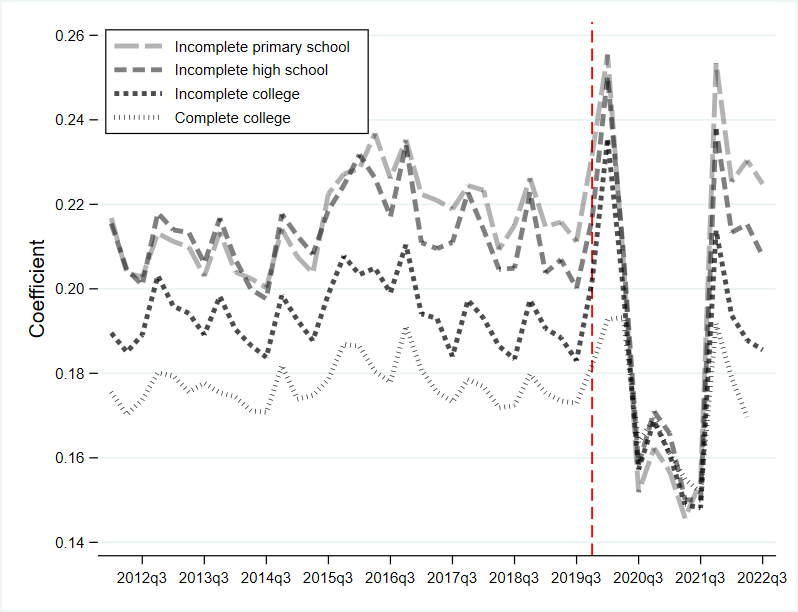
\includegraphics[width=0.85\linewidth]{../analysis/output/graph/_graph_regression_job_loss_determinants.png}
  \label{fig:_graph_regression_job_loss_determinants}
\end{figure}


\end{document}


